\subsection{Basis Transformation Rules}

\begin{figure}[h]
    \centering
    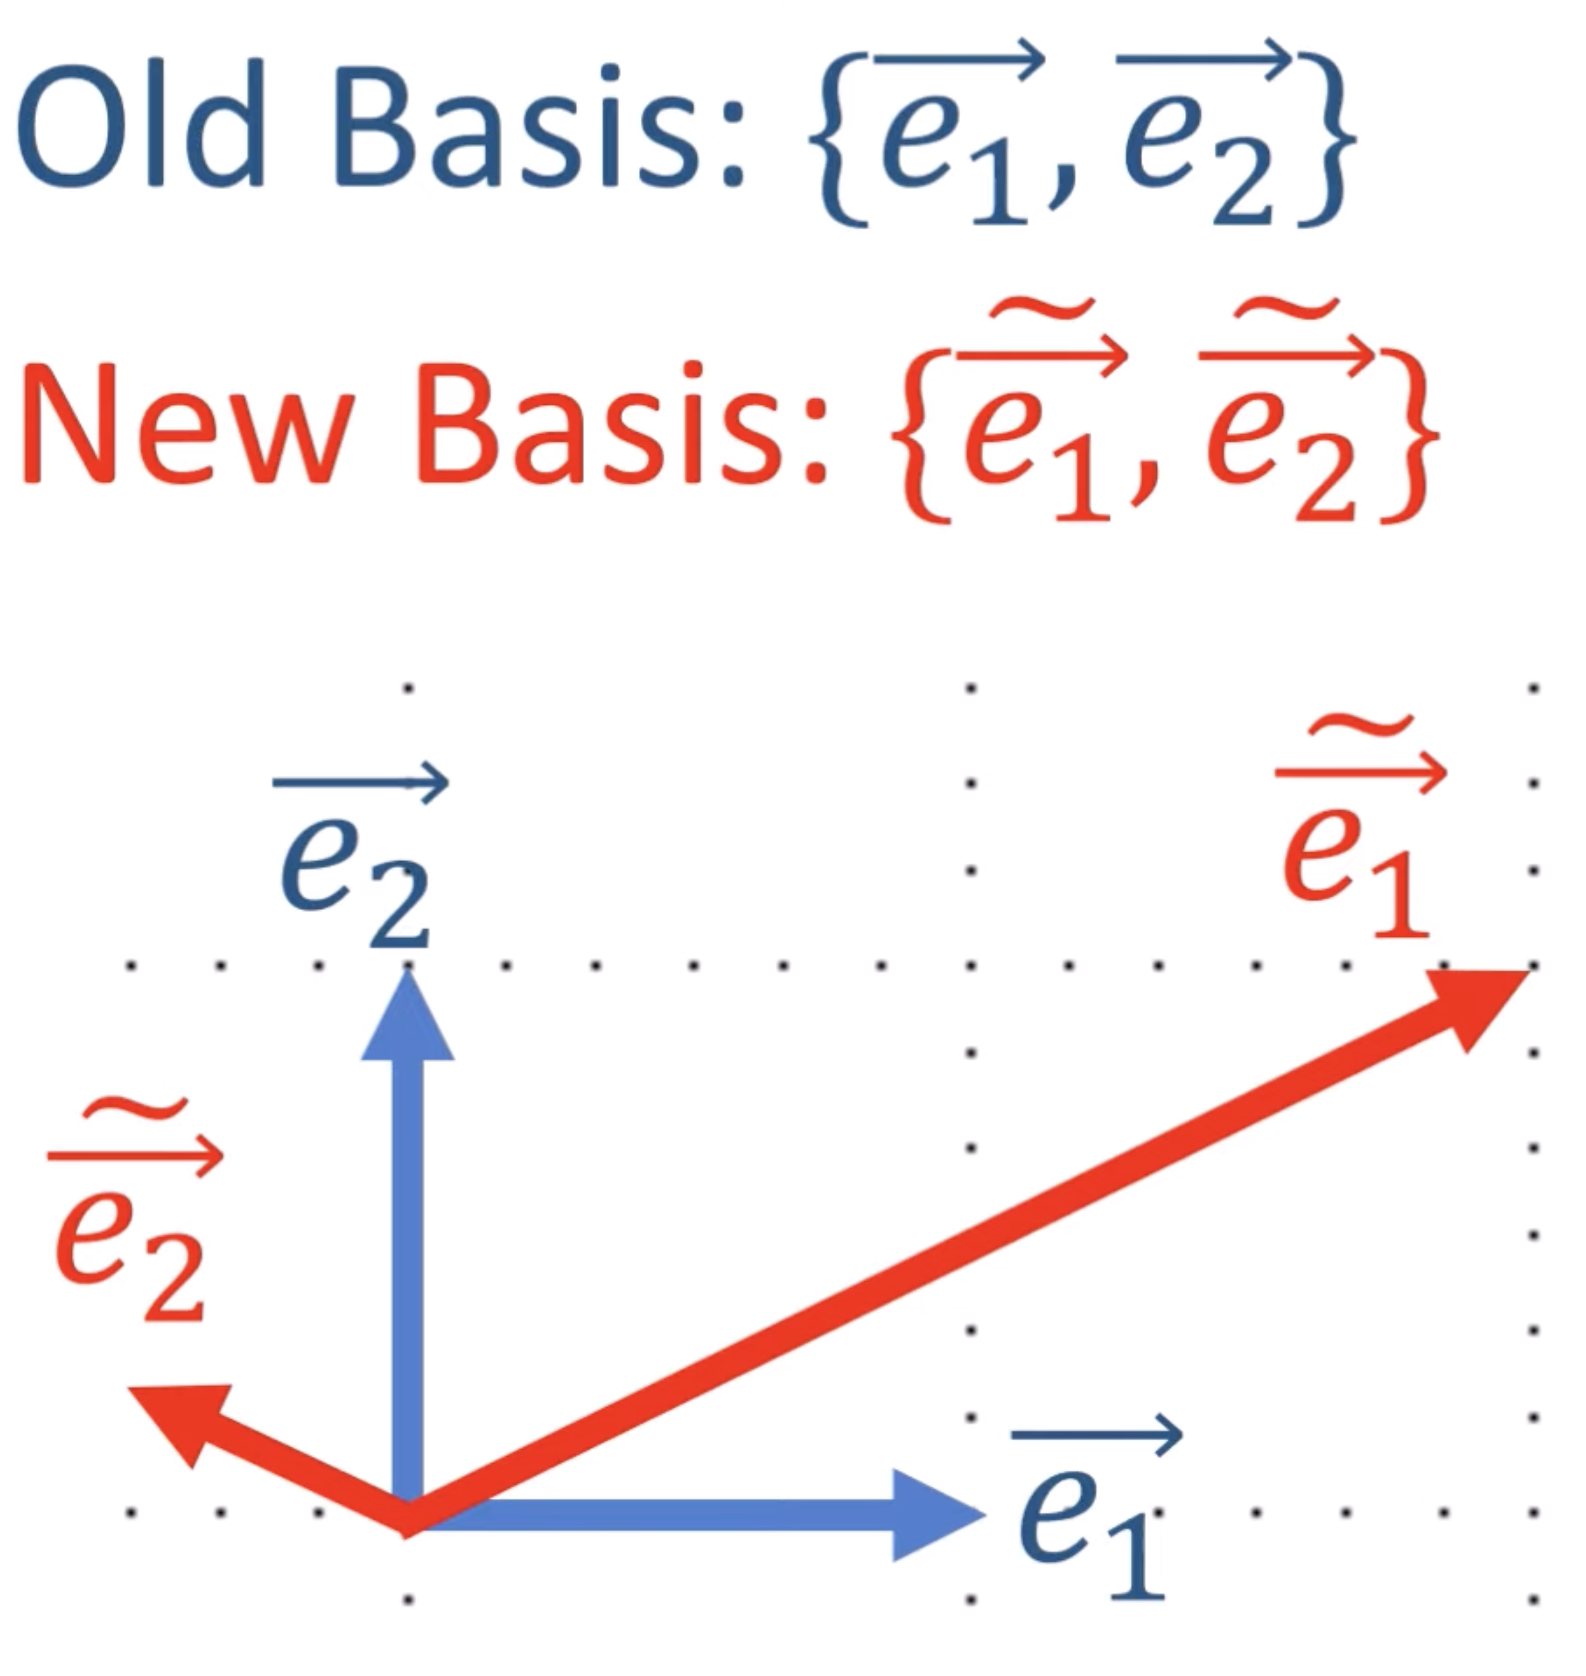
\includegraphics[width=0.25\textwidth]{Old_new_base_eigenchris}
    \caption{old and new basis vectors}
    \label{fig:old_new_base}
\end{figure}

\emph{Basis transformation:} The basis vectors of the new system expressed as a linear
combination of the basis vectors of the old system is considered a forward transformation.
The other direction is considered a backward transformation.\\

Here $F$ stands for $\underline{F}$orward transformation. Basis vectors are chosen to be
left multiplied to the transformation matrix, corresponding to summation via the first
index of the transformation matrix. Indices are chosen upper and lower to enable the
Einstein summation convention later on. Transformation indices are always from "north
west" to "south east":
\begin{equation}
    \label{eq:forward_trafo}
    \begin{array}{rcl}
        [\hdbtv{1} \quad \hdbtv{2}] & = &
        [\hdbv{1} \quad \hdbv{2}]
        \begin{bmatrix}
            F^{1~}_{~1} & F^{1~}_{~2} \\
            F^{2~}_{~1} & F^{2~}_{~2}
        \end{bmatrix} \\
        \noalign{\vskip10pt}
        \hdbtv{1} & = & F^{1~}_{~1}\hdbv{1} + F^{2~}_{~1}\hdbv{2}
        \quad \underset{\text{figure}~\ref{fig:old_new_base}}{=} \quad
        2 \hdbv{1} + 1 \hdbv{2} \\
        \hdbtv{2} & = & F^{1~}_{~2}\hdbv{1} + F^{2~}_{~2}\hdbv{2}
        \quad \underset{\text{figure}~\ref{fig:old_new_base}}{=} \quad
        -\frac{1}{2}\hdbv{1} + \frac{1}{4}\hdbv{2} \\
        \noalign{\vskip10pt}
        \Rightarrow \hdbtvc{j} & = &
        F^{k~}_{~j} \hdbvc{k} \quad\text{(summation convention)}
    \end{array}
\end{equation}

Here $B$ stands for $\underline{B}$ackward transformation:
\begin{equation}
    \label{eq:backward_trafo}
    \begin{array}{rcl}
        [\hdbv{1} \quad \hdbv{2}] & = &
        [\hdbtv{1} \quad \hdbtv{2}]
        \begin{bmatrix}
            B^{1~}_{~1} & B^{1~}_{~2} \\
            B^{2~}_{~1} & B^{2~}_{~2}
        \end{bmatrix} \\
        \noalign{\vskip10pt}
        \hdbv{1} & = & B^{1~}_{~1}\hdbtv{1} + B^{2~}_{~1}\hdbtv{2}
        \quad \underset{\text{figure}~\ref{fig:old_new_base}}{=} \quad
        \frac{1}{4} \hdbtv{1} + (-1) \hdbtv{2}\\
        \hdbv{2} & = & B^{1~}_{~2}\hdbtv{1} + B^{2~}_{~2}\hdbtv{2}
        \quad \underset{\text{figure}~\ref{fig:old_new_base}}{=} \quad
        \frac{1}{2}\hdbtv{1} + 2 \hdbtv{2} \\
        \noalign{\vskip10pt}
        \Rightarrow \hdbvc{i} & = &
        B^{j~}_{~i}\hdbtvc{j}\quad\text{(summation convention)}
    \end{array}
\end{equation}

Between $B$ and $F$ following relation holds:
\begin{equation}
    \label{eq:forward_backward_inverse}
    \begin{array}{rcl}
        B^{j~}_{~i} F^{k~}_{~j} & = & F^{k~}_{~j} B^{j~}_{~i}
        = \delta^k_i =
        \begin{cases}
            1, & \text{if}\ i = k \\
            0, & \text{if}\ i \neq k
        \end{cases} \\
        \text{full equation transposed:} & = &
        B^{i~}_{~j} F^{j~}_{~k} = \delta^i_k \\
        \noalign{\vskip10pt}
        \Rightarrow B & = & F^{-1} \quad\text{($B$ is the inverse of $F$)}
    \end{array}
\end{equation}


\newpage
